\section{Synchronous Distributed Systems}
\label{chap:3}

A synchronous distributed system is ..... TBC

A synchronizer is a general technique to simulate synchronous communication by asynchronous systems. Synchronizer was introduced by Awerbuch \cite{awerbuch1985complexity}, in this paper, the author presented 3 different synchronizers and analysed the trade off between them. This technique allows the execution of distributed synchronous algorithm over an asynchronous system, for instance, an asynchronous message passing system. The reason why synchronous algorithms are desirable is that there are usually simpler to design and superior in complexity. 

The graphic \ref{fig:simulation} shows the interactions between the layers of the simulation. The bottom layer is the asynchronous message passing system, here there is no guarantee on messages delay. A Synchronizer work over this layer. The goal of a synchronizer is to provide the illusion of synchronous system to the upper layer. For this example, the Maximal Independent Set algorithm is the user of the synchronizer. Any layer over the synchronizer can use the primitives \textit{Sync-}$send_i$ and \textit{Sync-}$recv_i$ and safely assume that the communication is synchronous.      

\begin{figure}[ht]
\centering
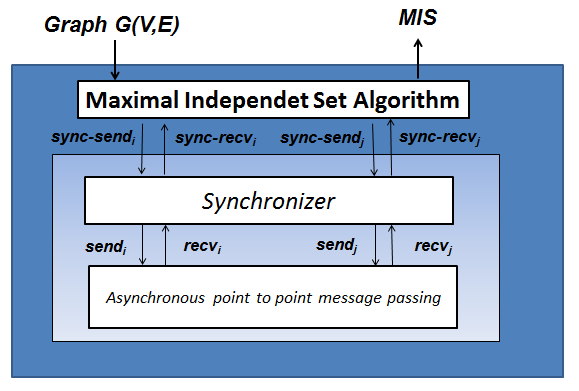
\includegraphics[width=1 \linewidth, height=8cm]{simulation.PNG} 
\caption{Diagram of the simulation of a synchronous distributed systems using synchronizers}
\label{fig:simulation}
\end{figure}


The following model was used in the original paper by Awerbuch \cite{awerbuch1985complexity} and was previously used in \cite{segall1983distributed,gallager1982distributed} among others. The asynchronous system is represented by an undirected graph $G = (V,E)$ where $V$ represent the set of processors and $E$ represent a bi-directional communication channel. Each processor sends messages, receive messages and perform some local computation. There is no notion of how long takes messages to arrive the destination but it is assumed to be finite. Another important assumption of the model is that the amount of information carried by messages is limited.

In this model, processes send messages after they receive a pulse or clock. This pulse represents one time unit (round) in the synchronous system. The delay of the messages in one round is one unit of time of the global clock.

\begin{definition}
\label{def:safe}
A process $p_i$ is said to be safe in a round only after all its messages has been delivered at their destinations.
\end{definition}

If all neighbours of $p_i$ are safe in the round $r$, this mean that $p_i$ has received all messages for $r$. In this case, $p_i$ in ready to execute the $r + 1$ round of the algorithm. This property ensures that from the point of view of the algorithm (that use the synchronizer), the network behaves as a synchronous communication system when really its an asynchronous system, this is why it is call a simulation. An easy solution to detect if a process is safe it is to force each process to acknowledge every message that receives. 

The  overhead generate by a Synchronizer $S$ with the acknowledgement mechanism is in the simplest case the double the number of messages of the original algorithm $A$. To compute the total message and time complexity of a synchronous algorithm it is necessary to sum the complexity of $A$ and $S$. $T(S)$ and $M(S)$ denote the time and message complexity respectively for a given synchronizer per round. If the synchronizer require an initialization phase (for instance, the Beta synchronizer used in this project) $T_{init}(S)$ and $M_{init}(S)$ express the message and time complexity of the initialization phase. The notation for the time and message complexity of the algorithm $A$ are $M(A)$ and $T(A)$. The total message complexity is then expressed by the equation \ref{ec:mess} and the time complexity by the equation \ref{ec:time}. 


\begin{equation}
\label{ec:mess}
 T_{tot} = T_{init}(S) + T(A)(1+T(S)) 
\end{equation}

\begin{equation}
\label{ec:time}
M_{tot} = M_{init}(S) + M(A) + T(A)M(S) 
\end{equation}


The two synchronizers presented in the next section are denoted Synchronizer $\alpha$ and Synchronizer $\beta$, which are a generalisation of a technique proposed by Gallager in \cite{gallager1982distributed}. These two synchronizer present a trade off between messages and time complexity. Synchronizer $\alpha$ is efficient in time but produce a significant overhead in message, while synchronizer $\beta$ has a better performance in communication but it is worse in time complexity.  



\subsection{Alpha Synchronizer}

One design challenge with synchronizers is that there are no bounds on messages delay, in consequence, a process cannot detect when is safe just waiting until receive all messages for a round because it will not know when all messages are receive. The Alpha synchronizer, proposed is \cite{awerbuch1985complexity} use the acknowledgement mechanism to solve this problem. 

In the Synchronizer $\alpha$, a process $p_i$ use the acknowledgement mechanism to detect if its safe with respect to the current round before start the next round. When $p_i$ detect that its safe then send a message <safe,round> to all its neighbours and after $p_i$ learns that all its neighbours are safe then start a new round.

The code for Synchronizer $\alpha$ is described in algorithm \ref{algorithm:alpha}, this code was extracted from \cite{attiya2004distributed}. 



\begin{algorithm}
 \caption{Alpha Synchronizer, code for $p_i$ from $i = 1$ to $N$}
 \label{algorithm:alpha} 

\SetAlgoNoLine

Initially round = 0 and \newline
\textit{buffer[r], safe[r]} and \textit{ack-missing[r]} are empty for all $r \geq 1$ \newline

\textbf{When} \textit{Synch-}$send_i$ (S) occurs:\newline
$round = round + 1$ \newline
\textit{ack-missing[round]} = {$j:p_j$ is a recipient of a message in S} \newline
enable \textit{Asynch-}$send_i(<m,round>)$  to $p_j$, for each $m \in S$ with recipient $p_j$ \newline

\textbf{When} \textit{Asynch-}$recv_i(<ack,r>)$ from $p_j$ occurs: \newline
add $(m,j)$ to \textit{buffer[r]} \newline
enable-$Asynch-send_i(<ack,r>)$ to $p_j$ \newline

\textbf{When} \textit{Asynch-}$recv_i(<ack,r>)$ from $p_j$ occurs: \newline
remove \textit{j} from \textit{ack-missing[r]} \newline
\If{ack-missing[r] = 0}{ 
enable \textit{Asynch-}$send_i(<safe,r>)$ to all neighbours \newline
}

\textbf{When} \textit{Asynch-}$recv_i(<safe,r>)$ from $p_j$ occurs: \newline
add \textit{j} to \textit{safe[r]} \newline
\If{safe[r] includes all neighbours}{
  enable \textit{Synch-}$recv_i(buffer[r])$ \newline
}

\end{algorithm}


The equation \ref{ec:message-alpha} describe the message complexity of Synchronizer $\alpha$, this is because in each round $p_i$ send extra messages to each neighbour. For this synchronizer, one additional time unit needs $p_i$ in order to detect that it is safe, therefore the time complexity is constant, see equation \ref{ec:time-alpha}. 


\begin{equation}
\label{ec:message-alpha}
 C(\alpha) = O(E) = O(V^2) 
\end{equation}

\begin{equation}
\label{ec:time-alpha}
 T(\alpha) = O(1) 
\end{equation}


\subsection{Beta Synchronizer}

Synchronizer $\beta$, also proposed in \cite{awerbuch1985complexity}, needs an initialization phase in which a rooted spanning tree is constructed over the network topology. A leader $S$ has to be chosen and then construct the spanning tree from the root. This synchronizer operates similar to Alpha Synchronizer regarding the acknowledgement process. When $p_i$ is safe inform its parents in a process call convercast. A process $p_i$ is safe if has received acknowledgement for each message in the actual round and receive safe from all its children in the spanning tree topology. Clearly this process needs to start in the leaves of the spanning tree. When the root is safe then broadcast OK and every process is allowed to pursue with the next round. This blow up the time overhead since the the mechanism act as a global synchronizer with a central leader, the process acting as a root of the spanning tree. 


\begin{algorithm}
 \caption{Beta Synchronizer, code for $p_i$ from i = 1 to N}
 \label{algorithm:beta} 

\SetAlgoNoLine

Compute a rooted spanning tree
Initially round = 0 and \newline
\textit{buffer[r], safe[r]} and \textit{ack-missing[r]} are empty for all $r \geq 1$ \newline

\textbf{When} \textit{Synch-}$send_i$ (S) occurs:\newline
$round = round + 1$ \newline
\textit{ack-missing[round]} = {$j:p_j$ is a recipient of a message in S} \newline
enable \textit{Asynch-}$send_i(<m,round>)$  to $p_j$, for each $m \in S$ with recipient $p_j$ \newline

\textbf{When} \textit{Asynch-}$recv_i(<ack,r>)$ from $p_j$ occurs: \newline
add $(m,j)$ to \textit{buffer[r]} \newline
enable-$Asynch-send_i(<ack,r>)$ to $p_j$ \newline

\textbf{When} \textit{Asynch-}$recv_i(<ack,r>)$ from $p_j$ occurs: \newline
remove \textit{j} from \textit{ack-missing[r]} \newline
\If{ack-missing[r] = 0}{ 
enable \textit{Asynch-}$send_i(<safe,r>)$ my parent in the spanning tree \newline
}
\If{$p_i$ is the root}{ 
enable \textit{Asynch-}$send_i(<go,r>)$ all $p_i$ children in the spanning tree \newline
}

\textbf{When} \textit{Asynch-}$recv_i(<go,r>)$ from $p_j$ occurs: \newline
  enable \textit{Synch-}$recv_i(buffer[r])$ \newline
  enable \textit{Asynch-}$send_i(<go,r>)$ all $p_i$ children in the spanning tree \newline

\end{algorithm}

The convercast and broadcast take at most $N - 1$ time units because the diameter of the spanning tree is $N - 1$, that gives $2N - 2$ combined. Time and message complexity and message complexity per synchronous round are expressed in the equations \ref{ec:message-beta} and \ref{ec:time-beta} respectively. The initialization phase only needs to be done one time for each topology, for this reason it is more interesting the overheads $T(\beta)$ and $M(\beta)$. The expression for the time and message complexity of the initialization phase are $T_{init}(\beta) = O(V)$ and $M_{init}(\beta) = O(M + N \log N)$ 

\begin{equation}
\label{ec:message-beta}
 C(\beta) = O(V)
 \end{equation}

\begin{equation}
\label{ec:time-beta}
 T(\beta) = O(V) 
\end{equation}

\subsection{Discussion about Synchronisation techniques}

One of the synchronizer is efficient in terms of time and the others in term of messages. The same author propose \cite{awerbuch1985complexity} another synchronizer that tries to get a low overhead in both, the Synchronizer $\gamma$ . Essentially, the idea is to generate a spanning forest of the graph and run beta synchronizer within each tree and alpha between trees. If there aren't too many adjacent trees message overhead is similar to the Beta Synchronizer. The time overhead is proportional to the depth of the trees. In some special cases  (depending on the topology of the graph, for instance a ring of k-cliques \cite{lynch1996distributed}), the Gamma Synchronizer can give similar cost as the original synchronous algorithm. However, it is also possible that the spanning forest need to be tuned for some kinds of graphs. Another drawback for the this synchronizer is the complexity of the implementation and the initialization phase that is more complex than the others. 

All these synchronizers require that the entire network participate in the synchronization process. As a result the overhead is always linear on the number of processors. The problem is when $p_i$ do not send any messages in one round, then any process $p_j$ that is neighbour of $p_i$ cannot deduce this because the delays in asynchronous networks are unbounded, in consequence, the use of timers are not useful. Awerbuch and Peleg proposed in \cite{awerbuch1990network} a poly-logarithmic overhead synchronizer based on involving the relevant portion of the topology in the synchronization process. However, it is possible that the synchronizer requiere high space complexity. Another approach for dynamic networks can relay on compute for each node what neighbours are active in one round and apply a simple synchronizer. This approach study in \cite{AspnesW2007} require that each $p_i$ compute all neighbours before the execution of each round.

For this project, besides Beta and Alpha Synchronizers, another global technique was used. A master process $M$ is required and each active process must inform $M$ that has finished the computation for the actual round. Then $M$ is in charge of notified every active process that may start a new round. This generate a lot of computation in the master process, however, no unnecessary message are send by inactive process. In the case of the Distributed Maximal Independent Set problem, specially with the algorithms study in this project this behaviour is desirable because many process become inactive very quickly. The three techniques are used in the simulation and an analysis of the trade-off between them is presented.

\newpage



